
\documentclass[12pt]{article}
\usepackage{graphicx}

\begin{document}

\begin{center}
\textbf{ MAT 442: HMW 1}\\
\end{center}

\textbf{1}. A population model is used in our scenario, which involves spruce budworm(tree-pest) and has a differential equation:
\begin{center}

y( $\psi$) = $ry(1-y/4)-Hy^2/y^2+A^2$  \hspace{2cm}(1.0)
\end{center}
 Looking at the equation above(1.0) there are four parameters namely r, K, H, A. In order to make graph plotting of our model easier, we adapt the rescaling procedure to change the dimension(number of parameters) for both population of spruce budworm and stipulated time that varies to particular threshold value.For instance, the number of spruce budworm versus needles in forest reserve which is a source of food for the spruce budworm, there is relative relationship between these two factors  because the more needles consumed by spruce budworm it depletes the forest hence shortage of food supply, we can also say the same for the opposite situation.The four parameters is scaled down from four to two and parameters in equation (1.0) are assigned new variables, hence  $x=y/k$ , $a=A/K$, t=($\psi$/1/r), $h=H/Hc$ .The following steps shows how rescaled model is obtained:

 
 \[\frac{dy}{d(\psi)}= \frac{dy}{d(x)} *\frac{dx}{d(t)}*\frac{dt}{d(\psi)}\]    
For left hand side(LHS):
\[ r* \frac{dx}{d(t)}*r \]  
For right hand side(RHS):
\[ r* kx(1-x)-\frac{Hx^2k^2}{(x^2)k^2+A^2} \]  
\[ r* kx(1-x)-\frac{Hx^2k^2}{(x^2)k^2+A^2/k^2} \]  
Therefore,  LHS=RHS this implies:
\[ r* k\frac{dx}{d(t)}= r* kx(1-x)-\frac{Hx^2k^2}{(x^2)k^2+A^2} \]  
Hence, \[\frac{dx}{d(t)} = x(1-x)-\frac{h}{4}\frac{x^2}{x^2+a^2} \]  



\cleardoublepage        



\textbf{2}. The following graphs are the reproduce Figures 2.4, 2.5 and 2.12 on pages 33 and 36 in our textboook.
\begin{figure} [ht!]
 \centering
 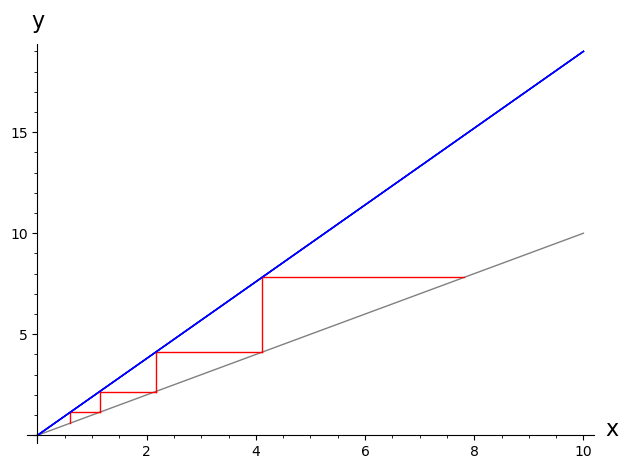
\includegraphics[height=2in]{/Users/ERICAGYEMANG/Desktop/Biomath/Figures/tmp.jpg} 
\caption[Figure 2.4: r>1]{Cobwebbing Method, $r>1$}
 \label{fig::model}
\end{figure}

\begin{figure} [ht!]
 \centering
 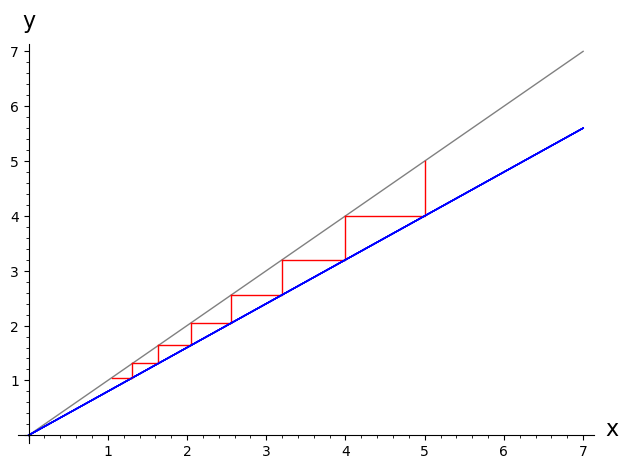
\includegraphics[height=2in]{/Users/ERICAGYEMANG/Desktop/Biomath/Figures/tmp1.jpg} 
\caption[Figure 5]{Cobwebbing Method, $0<r<1$}
 \label{fig::model}
\end{figure}  
 
 
 \cleardoublepage       
 
\begin{figure} [ht!]
 \centering
 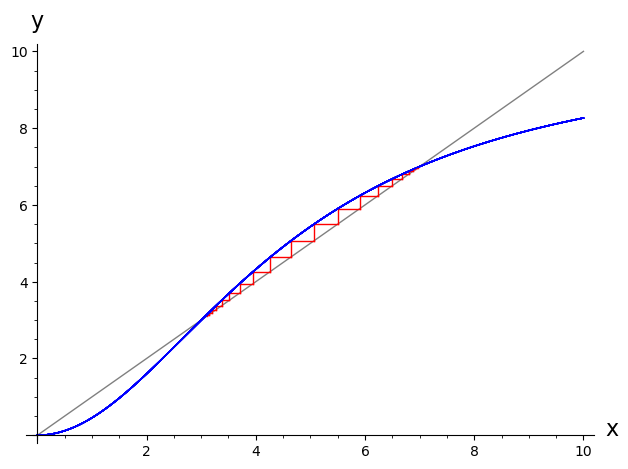
\includegraphics[height=2in]{/Users/ERICAGYEMANG/Desktop/Biomath/Figures/tmp2.jpg} 
\caption[Figure 5]{Cobwebbing Method, $r>2\sqrt{A}$}
 \label{fig::model}
\end{figure}   
 
 \cleardoublepage        
 
 
 \appendix
\section{Appendix}
 \subsection{Codes}
 
 def recur(f, x0, n):\\ 
    points = [(0, x0)] \\
    for i in [1..n]:
        points.append((i, f(points[i-1][1])))\\ 
    return points\\
f(x) = 2.1*x\\
def snail(f,x,u0,n,xmin,xmax): \\
    u = u0\\
    P = plot(x, x, xmin, xmax, color='gray')\\ 
    for i in range(n):\\
        P += line([[u,u],[u,f(u)],[f(u),f(u)]], color = 'red')\\ 
        u = f(u)\\
        P += f.plot(x, xmin, xmax, color='blue')\\
    P.show() \\
snail(f,x,0.5,4,0,10)\\

 
 \subsection{Codes}
 def recur(f, x0, n):\\ 
    points = [(0, x0)] \\
    for i in [1..n]:
        points.append((i, f(points[i-1][1])))\\ 
    return points\\
f(x) = 0.7*x\\
def snail(f,x,u0,n,xmin,xmax): \\
    u = u0\\
    P = plot(x, x, xmin, xmax, color='gray')\\ 
    for i in range(n):\\
        P += line([[u,u],[u,f(u)],[f(u),f(u)]], color = 'red')\\ 
        u = f(u)\\
        P += f.plot(x, xmin, xmax, color='blue')\\
    P.show() \\
snail(f,x,0.9,6,0,10)\\

\subsection{Codes}
def recur(f, x0, n):\\ 
    points = [(0, x0)] \\
    for i in [1..n]:
        points.append((i, f(points[i-1][1])))\\ 
    return points\\
f(x) = $10*x^2/(x^2+1)$\\
def snail(f,x,u0,n,xmin,xmax): \\
    u = u0\\
    P = plot(x, x, xmin, xmax, color='gray')\\ 
    for i in range(n):\\
        P += line([[u,u],[u,f(u)],[f(u),f(u)]], color = 'red')\\ 
        u = f(u)\\
        P += f.plot(x, xmin, xmax, color='blue')\\
    P.show() \\
snail(f,x,3.2,9,0,10)\\
 
                           
\end{document}
